\documentclass[a4paper,10pt]{article}

\usepackage[utf8]{inputenc} %
\usepackage[english]{babel}
\usepackage{fontenc}
\usepackage{graphicx}
\usepackage{amsfonts}
\usepackage{hyperref}
\usepackage{amssymb}
\usepackage{fullpage}
% \usepackage[ruled,vlined,linesnumbered]{algorithm2e}
\usepackage{float}
\usepackage{amsthm}
\usepackage{amsmath}
\usepackage{amssymb}
\usepackage{mathrsfs}
\usepackage{enumerate}
% \usepackage{wrapfig}
% \providecommand{\SetAlgoLined}{\SetLine}
% \providecommand{\DontPrintSemicolon}{\dontprintsemicolon}
\author{M1-MPRI Projet Génie Logiciel}
\date{Le 25/10/13}
\title{Délivrable I
}
% \theoremstyle{definition}
% \newtheorem{lemma}{Lemme}
% % \newtheorem{proposition}{Propriété}[chapter]
% % \newtheorem{definition}{Définition}[chapter]
% % \newtheorem{example}{Exemple}[chapter]
% % \newtheorem{cor}{Corollaire}[chapter]
% % \newtheorem{theorem}{Théorème}[chapter]
% \theoremstyle{definition}
\usepackage{tikz}
\usetikzlibrary{arrows}
\usepackage{fullpage}
\usepackage{empheq}
%  
% \newlength\dlf  % Define a new measure, dlf
% \newcommand\alignedbox[2]{
% % Argument #1 = before & if there were no box (lhs)
% % Argument #2 = after & if there were no box (rhs)
% &  % Alignment sign of the line
% {
% \settowidth\dlf{$\displaystyle #1$} 
%     % The width of \dlf is the width of the lhs, with a displaystyle font
% \addtolength\dlf{\fboxsep+\fboxrule} 
%     % Add to it the distance to the box, and the width of the line of the box
% \hspace{-\dlf} 
%     % Move everything dlf units to the left, so that & #1 #2 is aligned under #1 & #2
% \boxed{#1 #2}
%     % Put a box around lhs and rhs
% }
% }
% \theoremstyle{remark}
% % \newtheorem{req}{Remarque}[chapter]
% % \newtheorem{nota}{Notation}[chapter]

\tikzset{
    punkt/.style={
           rectangle,
           rounded corners,
           draw=black, very thick,
           text width=5em,
           minimum height=2em,
           text centered},
               punkt2/.style={
           rectangle,
           draw=pink, very thick,
           text width=5em,
           minimum height=2em,
           text centered},
  punktsi/.style={
           rectangle,
           rounded corners,
           draw=green, very thick,
           text width=5em,
           minimum height=2em,
           text centered},
             punktre/.style={
           rectangle,
           rounded corners,
           draw=blue, very thick,
           text width=5em,
           minimum height=2em,
           text centered},
             punktsc/.style={
           rectangle,
           rounded corners,
           draw=cyan, very thick,
           text width=5em,
           minimum height=2em,
           text centered},
             punktgr/.style={
           rectangle,
           rounded corners,
           draw=magenta, very thick,
           text width=5em,
           minimum height=2em,
           text centered},
             punktge/.style={
           rectangle,
           rounded corners,
           draw=yellow, very thick,
           text width=5em,
           minimum height=2em,
           text centered},
             punktmu/.style={
           rectangle,
           rounded corners,
           draw=red, very thick,
           text width=5em,
           minimum height=2em,
           text centered},
  treenode/.style = {align=center, inner sep=0pt, text centered,
    font=\sffamily},
  arn_n/.style = {treenode, circle , white, font=\sffamily\bfseries, draw=black,
    fill=black, text width=1.5em},% arbre rouge noir, noeud noir
  arn_r/.style = {treenode, circle , red, draw=red, 
    text width=1.5em, very thick},% arbre rouge noir, noeud rouge
  arn_x/.style = {treenode, rectangle, draw=black,
    minimum width=1em, minimum height=1em},% arbre rouge noir, nil
  arn_b/.style = {treenode, circle , blue, draw=blue, 
    text width=1.5em, very thick},
  arn_g/.style = {treenode, circle , green, draw=green, 
    text width=1.5em, very thick},
  arn_y/.style = {treenode, circle , yellow, draw=yellow, 
    text width=1.5em, very thick},
    arn_pu/.style = {treenode, circle , purple, draw=purple, 
    text width=1.5em, very thick},
    arn_pi/.style = {treenode, circle , pink, draw=pink, 
    text width=1.5em, very thick},
    arn_rb/.style = {treenode, circle , red, draw=red, 
    text width=2.5em, very thick}
    }% arbre rouge noir, noeud rouge}
    
\begin{document}
\maketitle
\tableofcontents

\section{Introduction}
\section{Architecture générale}
\subsection{Les différentes composantes et leurs interfaces}
% \begin{figure}[h]
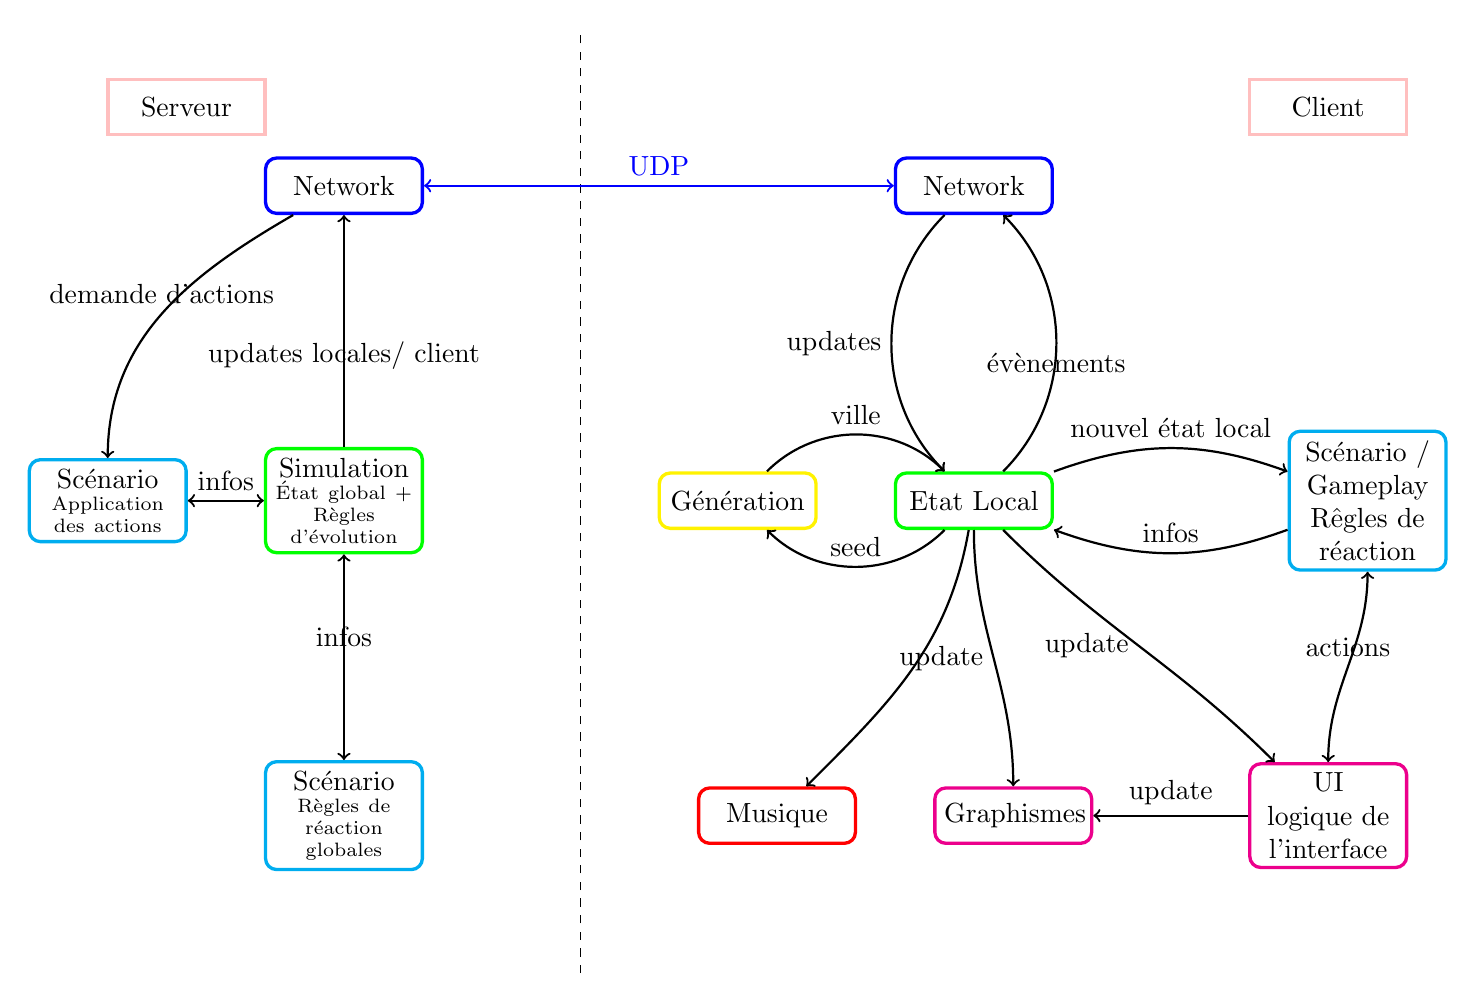
\begin{tikzpicture}
      \node[punktsi] (0) at (3,0) {Etat Local};
      \node[punktge] (1) at (0,0) {Génération};
      \node[punktmu] at (0.5,-4) (2) {Musique};
      \node[punktgr] at (3.5,-4) (3) {Graphismes};
      \node[punktgr] at (7.5,-4) (4) {UI \\ logique de l'interface};
      \node[punktsc] at (8,0) (5) {Scénario / Gameplay \\ Rêgles de réaction};
      \node[punktre] at (3,4) (6) {Network};
      \node[punktsi] at (-5,0) (7) {Simulation \\ {\scriptsize État global + \\ Règles d'évolution\\}};
      \node[punktsc] at (-5,-4) (8) {Scénario \\ {\scriptsize Règles de réaction globales\\}};
      \node[punktre] at (-5,4) (10) {Network};
      \node[punkt2] at (7.5,5) {Client};
      \node[punkt2] at (-7,5) {Serveur};
      \node[punktsc] at (-8,0) (11){Scénario \\ {\scriptsize Application des actions\\}};
      \draw[-,black,dashed] (-2,-6) -- (-2,6);
      \draw[->,black,thick] (1) to[out=45,in=135] node [midway,above] {ville} (0);
      \draw[->,black,thick] (0) to[out=225,in=-45] node [midway,above] {seed} (1);
      \draw[->,black,thick] (0) to[out=260,in=45] (2);
      \draw[->,black,thick] (0) to[out=270,in=90] node [midway,left] {update} (3);
      \draw[->,black,thick] (0) to[out=-45,in=135] node [midway,left] {update} (4);
      \draw[->,black,thick] (0) to[out=20,in=160] node [midway,above] {nouvel état local} (5);
      \draw[->,black,thick] (5) to[out=200,in=-20] node [midway,above] {infos} (0);
      \draw[<->,black,thick] (4) to[out=90,in=-90] node [midway,above] {actions} (5);
      \draw[->,black,thick] (4) to[out=180,in=0] node [midway,above] {update} (3);
      \draw[->,black,thick] (0) to[out=45,in=-45] node [midway,below] {évènements} (6);
      \draw[->,black,thick] (6) to[out=-135,in=135] node [midway,left] {updates} (0);
      \draw[<->,blue,thick] (6) to[out=180,in=0] node [midway,above] {UDP} (10);
%       \draw[->,black,thick] (10) to[out=-135,in=135] node [midway,above] {actions client} (7);
      \draw[->,black,thick] (7) to node [midway,below] {updates locales \\ / client} (10);
      \draw[<->,black,thick] (8) to[out=90,in=-90] node [midway,above] {infos} (7);
      \draw[<->,black,thick] (11) to[out=0,in=180] node [midway,above] {infos} (7);
      \draw[<-,black,thick] (11) to[out=90,in=-150] node [midway,above] {demande d'actions} (10);
\end{tikzpicture}
% \caption{Structure \& interactions des composantes}
% \end{figure}

\begin{figure}[h]
\centering
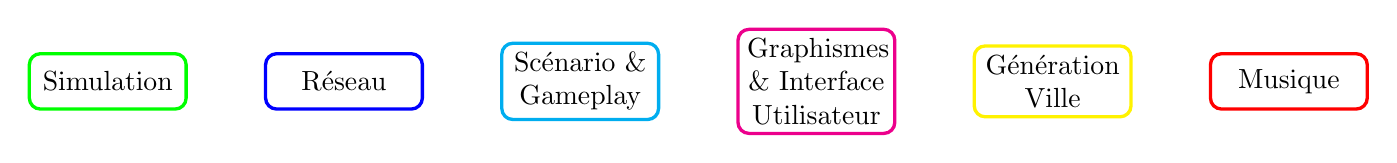
\begin{tikzpicture}
\node[punktsi] at (0,0) {Simulation};
\node[punktre] at (3,0) {Réseau};
\node[punktsc] at (6,0) {Scénario \& Gameplay};
\node[punktgr] at (9,0) {Graphismes \& Interface Utilisateur};
\node[punktge] at (12,0) {Génération Ville};
\node[punktmu] at (15,0) {Musique};
\end{tikzpicture}
 \caption{Code couleur des différents groupes de travail}
\end{figure}
\section{Description des sous projets}
\subsection{Simulation}
\subsection{Réseau}
\subsection{Scénario \& Gameplay}
\subsection{Graphismes \& Interface Utilisateur (IU)}
\subsection{Génération ville}
\subsection{Musique}

\end{document}